\chapter{Algoritmo de Shor}
El algoritmo de Shor es un AC de factorización de enteros. Dado un entero $N=p \times q$, donde $p$ y $q$ son primos, el algoritmo de Shor encuentra $p$ y $q$ en $O((\log(N))^3)$ pasos. El algoritmo clásico más eficiente para factorizar enteros es la cibra general del cuerpo de números y funciona con una complejidad heurística de $O(e^{(\sqrt[3]{\frac{64}{9}}+o(1))(\ln(N))^{\frac{1}{3}}(\ln(\ln(N)))^{\frac{2}{3}}})$. Por su capacidad de factorizar números semiprimos, el algoritmo de Shor es capaz de violar el cifrado RSA y el protocolo Diffie-Hellman de intercambio de llaves, sobre los cuáles se basa virtualmente toda la criptografía actual.

\section{Estimación de orden}

Dado $m \in \mathds{N}$, se dice que $a,b \in \mathds{Z}$ son congruentes módulo m si y sólo si $(a-b)/m \in \mathds{Z}$.

\begin{enumerate}
    \item Se denota por $a \equiv b \mod m$, siendo m el módulo de la congruencia.
    \item Si m divide a $(a-b)$, ambos a y b tienen el mismo resto al ser divididos por el módulo m.
\end{enumerate}

 Ejemplos:

\begin{align*}
    23 \equiv 2 \mod 7 &\rightarrow 23 = 3 \times 7 + 2 \\
    -6 \equiv 1 \mod 7 &\rightarrow -6 = -1 \times 7 +1
\end{align*}

 Además si $m \in \mathds{N}$ y $a,b,c,d \in \mathds{Z}$ tales que:

\begin{align*}
    a+c &\equiv b+d \mod m \\
    a c &\equiv b d \mod m
\end{align*}

 Por definición el orden $x \mod N$ es el menor entero r distinto de cero que satisface $x^r = 1 \mod N$
 
Ejemplo:

 Sea $x = 4, N = 13 \rightarrow 4^p = 13 q + R \qquad 4^p \mod 13 = R$

 \[\begin{matrix}
         p  &   4^p & 4^p = 13 q                         + R    &   R   \\
         0  &   1   & 4^0 = 13\times0                    + 1    & 1     \\
         1  &   4   & 4^1 = 13\times0                    + 4    & 4     \\
         2  &   16  & 4^2 = 13\times1                    + 3    & 3     \\
         3  &   64  & 4^3 = 13\times4                    + 12   & 12    \\
         4  &   256  & 4^4 = 13\times19                  + 9    & 9     \\
         5  &   1024  & 4^5 = 13\times78                 + 10   & 10    \\ % Revisar tabla | Error en la clase
         6  &   4096  & 4^6 = 13\times315                + 1    & 1     \\
         7  &   16384  & 4^7 = 13\times1260              + 4    & 4     \\
         8  &   65536  & 4^8 = 13\times5041              + 3    & 3     \\
         9  &   262144  & 4^9 = 13\times20164            + 12   & 12    \\
         10 &   1048576  & 4^10 = 13\times80659          + 9    & 9     \\
         11 &   4194304  & 4^11 = 13\times322638         + 10   & 10    \\
         12 &   16777216  & 4^12 = 13\times1290555       + 1    & 1     \\
         13 &   67108864  & 4^13 = 13\times5162220       + 4    & 4     \\
         14 &   268435456  & 4^14 = 13\times20648881     + 3    & 3     \\
         15 &   1073741824  & 4^15 = 13\times82595524    + 12   & 12    \\
         16 &   4294967296  & 4^16 = 13\times330382099   + 9    & 9     
     \end{matrix}
 \]

 Como podemos ver el período es r=6, el cual corresponde al menor r entero distinto de cero para el cual se cumple $4^r=1 \mod 13$ con r=6

 $\therefore 4^6 = 1 \mod 13$

\section{Expansión en fracciones contínues}

[(Emmanuel Desurvire -> Apéndice R)]

Definamos un número real $\chi_n = a_0 \frac{1}{a_1 + \frac{1}{a_2 + \frac{1}{a_3 + \frac{1}{... a_n}}}}$ con $n \leq N$. Cada número real en el conjunto $\{x_0,x_1,...,x_{N-1},x_N\}$ se denomina un convergente de $x_n$, mientras que $x_n$ se denomina el n-ésimo convergente de $x_n$.

Propiedad 1:

El conjunto finito $\{a_0,a_1,a_2,...,a_n\}$ de números reales positivos corresponde a la razón: $x_n = \frac{p_n}{q_n}$, donde los $p_n$ y $q_n$ son definidos como:

$p_n = a_n p_{n-1} + p_{n-2}$
$q_n = a_n q_{n-1} + q_{n-2}$

con $n \geq 2, p_0 = a_0, q_0 = 1, p_1 = 1 + a_0 a_1 y q_1 = a_1$, para n = 0, 1.

Propiedad 2:

Los números reales $p_n$, $q_n$ son coprimos y satisfacen la relación:

$q_n p_{n-1} - p_n q_{n-1} = (-1)^n)$

Propiedad 3:

Dado un número racional x, si dos enteros p, q son tales que:

$|\frac{p}{q} - x| \leq \frac{1}{2q^2}$

Entonces p/q es un convergente de x.

Asumamos como ejemplo:

$\phi = 711/413 = 1.72154963680387$

Entonces:

$\phi = 711/413 = 1 + \frac{1}{1 + \frac{1}{2 + \frac{1}{1 + \frac{1}{1 + \frac{1}{2 + \frac{1}{4 + \frac{1}{5}}}}}}}$

Supongamos que solo queremos 6 decimales de precisión, es decir sea $\tilde{\phi} = 1.721549$, tal que:

$|\epsilon = |\phi - \tilde{\phi}| = 3.699 10^{-7}$

Si expandimos $\tilde{\phi}$ al igual que $\phi$, encontramos que con sólo 7 $a_n$ encontramos $\tilde{\phi}$ (ver tabla R1).

Por otro lado, $\frac{p_7}{q_7} \implies \frac{711}{413}$ da la definición de $\phi$.

\section{Algoritmo de factorización de Shor}

El algoritmo de factorización de Shor permite factorizar números los cuales se pueden descomponer en un producto único de números primos.

Dicho número N es un entero no-primo de L bits.

En un ordenador cuántico el algoritmo de Shor tendrá un tiempo de corrida del orden $O((L^3))$ (polinómico) y en un ordenador clásico es del $O(e^[L^{1/3} (log L)^{2/3}])$ (exponencial), mostrando así que el algorimo de Shor es capaz de factorizar números muy grandes en tiempos polinómicos.

En dicho algoritmo se conjugan:

1. Aritmética modular <- Clásico
2. Paralelismo cuántico <- Cuántico
3. Transformada cuántica de Fourier <- Cuántico

El algoritmo consiste en dos etapas:

1) Una reducción del problema de descomponer en factores al problema de encontrar el orden

2) Un algoritmo cuántico para solucionar el problema de encontrar el período.

El algoritmo de Shor fue publicado en: P.W. Shor SIAM I. Comput. 26, 1484-1509 (1997(

Siguiendo el esquema de Emmanuel Desuvire "Classical and Quantum Information Theory: An Introduction for the Telecom Scientist".

La parte cuántica del algoritmo de Shor la podemos dividir en 2 partes:

1) El algoritmo de estimación de fase
2) El algoritmo de determinación de orden

Entonces:

\section{Estimación de fase}

Asumamos que tenemos un operador U, con autoestados $\ket{u}$ de dimensión L, y con autovalore complejos dessconocidos $\lambda_\phi = e^{2 i \pi \phi}$, donde $\phi$ es un número real tal que $0 \leq \phi \leq 1$, a ser determinado.

Asumamos también que somos capaces de construir una familia de operadores $controlled-U^p$, donde $p = 2^0, 2^1, 2^2, ..., 2^{k-1}$

El circuito cuántico del algoritmo de estimación de fase viene expresado en dos etapas, a las que llamaremos "front-end" y "back-end".

Analicemos la etapa front-end:

%%%%%% CIRCUITO AQUÍ %%%%%%

Recordemos que:

%C

Analicemos ls compuerta $CU^p \equiv controlled-U^p gate$:

%C

$U \ket{u} = e^{2 i \pi \phi}$
$U^p \ket{u} = e^{2 i \pi p \phi}$
$H \ket{0} = \ket{0} + \ket{1}$ (Sin $1\sqrt{2}$ por los momentos)

$CU^p ((\ket{0} + \ket{1}) \otimes \ket{u} = \ket{0} \otimes \ket{u} + \ket{1} \otimes U^p \ket{u} = \ket{0} \otimes \ket{u} + \ket{1} e^{2i \pi p \phi} \ket{u} = (\ket{0} + e^{2 i p \pi \phi}) \otimes \ket{u}$

$\therefore CU^p ((\ket{0} + \ket{1}) \otimes \ket{u}) = (\ket{0} + e^{2 i \pi p \phi} \ket{1}) \otimes \ket{u}$

Analicemos ahora el producto tensorial a la salida de dos compuertas $CU^p$ recordemos que $p = \{2^0, 2^1, ..., 2^{k-1}\}$, entonces:

$(\ket{0} + e^{2 i \pi 2^1 \phi} \ket{1}) \otimes (\ket{0} + e^{2 i \phi 2^0 \phi} \ket{1}) = \ket{0} \ket{0} + e^{2 i \pi 2^0 \phi} \ket{0} \ket{1} + e^{2 i \pi 2^1 p} \ket{1} \ket{0} + e^{2 \pi i (2^1 + 2^0) \phi} \ket{1} \ket{1} = e^{2 i \pi 0 \phi} \ket{0} + e^{2 i \pi 1 \phi} \ket{1} + e^{2 i \pi 2 \phi} \ket{2} + e^{2 i \pi 3 \phi} \ket{3}$

donde $\ket{00} \equiv \ket{0}; \ket{01} \equiv \ket{1}; \ket{10} \equiv \ket{2}; \ket{11} \equiv \ket{3};$

% revisar exponentes | error en la clase
es decir: $\ket{ij} \equiv \ket{i 2^0 + j 2^1}$ con i,j = 0,1
si generalizamos: $\ket{i j k ... n} = \ket{i 2^0 + j 2^1 + k 2^2 + ... + n 2^{n-1}}$

$\therefore (\ket{0} + e^{2 i \pi 2^1}) \otimes (\ket{0} + e^{2 i \pi 2^0 \phi} \ket{1}) = \sum\limits_{k = 0}^3 e^{2i \pi k \phi} \ket{k}$

Todo número puede ser representado en forma binaria:

$0 \leq \phi \leq 1 \implies \phi \equiv 0 \phi_1 \phi_2 \phi_3 ... \implies \phi = \frac{\phi_1}{2} + \frac{\phi_2}{4} + \frac{\phi_3}{8} + ... + \frac{\phi_k}{2^k} + ...$

para bits $\phi_i = 0,1 \rightarrow \phi_1 = 0 y \phi_2 = 1$

luego: .) $2^{k-1} \phi = 2^{k-1} ( \frac{\phi_1}{2} + \frac{\phi_2}{4} + \frac{\phi_3}{8} + ... + \frac{\phi_k}{2^k} + ...) = \{\phi_1 2^{k-2} + \phi_2 2^{k-3} + ... + \phi_{k-1} 2^0\} + \frac{\phi_k}{2} + \frac{\phi_{k-1}}{4} + ...$

.) $2^{k-2} \phi = 2^{k-2} ( \frac{\phi_1}{2} + \frac{\phi_2}{4} + \frac{\phi_3}{8} + ... + \frac{\phi_k}{2^k} + ...) = \{\phi_1 2^{k-3} + \phi_2 2^{k-4} + ... + \phi_{k-2} 2^0\} + \frac{\phi_{k-1}}{2} + \frac{\phi_k}{2} + \frac{\phi_{k+1}}{8} + ...$

Los términos dentro de los \{ \} son enteros. Definamos entonces:

$\Omega_m = \sum\limits_{l=1}^m \frac{\phi_{k-m+l}}{2^l}$

tal que:

$e^{2 i \pi 2^{k-1} \phi} = e^{2 i \phi \Omega_1} e^{2 i \pi (\frac{\phi_{k+1}}{4} + ...)}$
$e^{2 i \pi 2^{k-2} \phi} = e^{2 i \phi \Omega_2} e^{2 i \pi (\frac{\phi_{k+1}}{8} + ...)}$
.
.
.
$e^{2 i \pi 2^0 \phi} = e^{2 i \phi \Omega_k} e^{2 i \pi (\frac{\phi_{k+1}}{2^{k+1}} + ...)}$

Consideremos el caso en el cual $\phi$ es definido exactamente por k bits tal que $\phi_{k+1} = \phi_{k+2} = ... = 0$

Dejando de lado el qubit $\ket{u}$ la salida del primer registro es:

$\frac{1}{2^{k/2}} (\ket{0} + e^{2 i \pi \Omega_1} \ket{1}) \otimes (\ket{0} + e^{2 i \pi \Omega_2}) \otimes ... \otimes (\ket{0} + e^{2 i \pi \Omega_k} \ket{1})$

Como podemos recordar

$QFT \ket{n} = \frac{1}{2^{k/2}} (\ket{0}_1 + e^{2 i \pi \Omega_1} \ket{1}_1) \otimes (\ket{0}_2 +  e^{2 i \pi \Omega_2} \ket{1}_2) \otimes ... \otimes (\ket{0}_k + e^{2 i \pi \Omega_k} \ket{1}_k)$

Siendo: $1 \leq m \leq k \rightarrow \ket{m} = \frac{1}{2^{m/2}} (\ket{0}_m + e^{2 i \pi \Omega_m} \ket{1}_m)$

con $\Omega_m = \sum\limits_{l=1}^m \frac{n_{k-m+l}}{2}$

Encontrando así que $\frac{1}{2^{k/2}} (\ket{0} + e^{2 i \pi \Omega_1} \ket{1}) \otimes (\ket{0} + e^{2 i \pi \Omega_2} \ket{1}) \otimes ... \otimes (\ket{0} + e^{2 i \pi \Omega_k} \ket{1})$

Es la transformada cuántica de Fourier de nuestro estado $\ket{\phi}$ obtenida con las compuertas $Controlled-U^p$.

Al ket $\ket{\phi}$ lo podemos recuperar haciendo la transformada inversa de Fourier.

Consideremos ahora el módulo del circuito cuántico "back-end"

% C

El módulo back-end del circuito cuántico de Shor consiste en realizar la transformada cuántica inversa de Fourier y hacer medidas sobre los k qubits encontrando así los $\phi_1, \phi_2,...,\phi_k$.

Seguidamente consideremos ahora el caso más general en el cual $2^k \phi$ no es un entero.

Fron-end $\ket{0}^{\otimes k} \otimes \ket{u} \rightarrow \frac{1}{\sqrt{N}} \sum\limits_{k=0}^{N-1} e^{2 i \pi k \phi} \ket{k} \otimes \ket{u}$

Back-end $QFT_1^\dagger (\frac{1}{\sqrt{N}} \sum\limits_{k=0}^{N-1} e^{2 i \pi k \phi} \ket{k} \otimes \ket{u}) = \frac{1}{\sqrt{N}} \sum\limits_{k=0}^{N-1} e^{2 i k \phi} QFT^\dagger \ket{k} \otimes \ket{u} = \frac{1}{\sqrt{N}} \sum\limits_{k=0}^{N-1} e^{2 i \pi k \phi} (\frac{1}{2^{k/2}} \sum\limits_{n=0}^{N-1} e^{-\frac{2 \pi i k n}{N} \ket{n}) \ket{u} = \frac{1}{N} \sum\limits_{k=0}^{N-1} \sum\limits_{n=0}^{N-1} e^{- 2 \pi i \frac{k n}{N}} e^2 i pi k \phi} \ket{n} \otimes \ket{u} = \frac{1}{N} \sum\limits_{n=0}^{N-1} (\sum\limits_{k=0}^{N-1} (e^{2 i \pi (\phi - \frac{n}{N})})^k ) \ket{n} \otimes \ket{u}$

$\therefore (QFT^\dagger \otimes \mathds{1}) (\frac{1}{\sqrt{N}} \sum\limits_{k=0}^{N-1} e^{2 i \pi k \phi} \ket{k} \otimes \ket{u}) = \frac{1}{N} \sum\limits_{n=0}^{N-1} (\frac{1 - e^{2 i \pi (\phi - \frac{n}{N})N}}{1 - e^{2 i \pi (\phi - \frac{n}{N})}}) \ket{n} \otimes \ket{u}$

La probabilidad de medir n a la salida del registro será:

$p(n) = |\bra{u} \otimes \bra{n} \ket{\psi_{output}}|^2$

$p(n) = \frac{1}{N^2} |\frac{1 - e^{2 i \pi (\phi - \frac{n}{N})N}}{1 - e^{2 i \pi (\phi - \frac{n}{N})}}|^2$

$\therefore p(n) = \frac{1}{N^2} \frac{\sin^2(\pi (\phi - \frac{n}{N}) N)}{\sin^2(\pi (\phi - \frac{n}{N}))}$

La medida de n con probabilidad asociada p(n), corresponde a la estimación de fase $\tilde{\phi} = n/N$. La probabilidad es máxima cuando $\delta = \phi - \tilde{\phi}$ es mínima.

$p(n) = \frac{1}{N^2} \frac{\sin^2(\pi (\phi - \frac{n}{N}) N)}{\sin^2(\pi (\phi - \frac{n}{N}))}$ si N es grande $\rightarrow$ %Graf

La probabilidad p(n) decae rápidamente a cero cuando el error $\delta$ se aleja del mínimo.

Entonces:

.) La medida tiene la maor probabilidad de dar la aproximación más cercana al estado $\phi$.
.) El circuito de salida es de la forma $\ket{\tilde{\phi}} \ket{u}$, donde $\ket{\tilde{\phi}}$ es una superposición de estados, los cuales al medirlos dan una buena aproximación de $\phi$.

\section{Estimación de orden}

Analicemos como la estimación de fase hace posible determinr r, el orden de $x \mod N$, con alta probabilidad y precisión.

Primero necesitamos introducir el operador U y sus correspondientes autovectores y autovalores.

Asumamos que dados dos enteros x y N que satisfacen que x<N, siendo x coprimo de M, es decir mcd(x,M)=1, existe un operador $U_{x,N}$ que actúa sobre el qubit $\ket{y} \equiv \{\ket{0}, \ket{1}\}$, tal que:

$U_{x,N} \ket{y} = \ket{x y \mod N}$

Asumamos $\{ \ket{u_s}\}_{s = 0, 1, ..., r-1}$ el conjunto de r autoestados de U, asociados con los autovalores $e^{i 2 \pi s/r}$ tal que $U \ket{u_s} = e^{2 i \pi s /r} \ket{u_s}$ en el cual la fase es $\phi_s = s/r$ con $0 \leq \phi_s \leq 1$

Tales autoestados $\ket{u_s}$ se definen acorde a: $\ket{u_s} = \frac{1}{\sqrt{r}} \sum\limits_{k=0}^{r-1} e^{\frac{-2 i \pi k s}{r}} \ket{x^k \mod N}$, siendo r a determinar.

Con las siguientes propiedades:

$\frac{1}{\sqrt{r}} \sum_{s=0}{r-1} \ket{u_s} = \ket{1}$

$\frac{1}{\sqrt{r}} \sum\limits_{s=0}^{r-1} e^{\frac{2 i \pi k s}{r}} \ket{u_s} = \ket{x^k \mod N}$

$p(s) = |c_s|^2 = \frac{1}{r}$

El circuito para la estimación de orden es el siguiente:

%%%%%% Circuito aqui%%%%%%

Entonces:

$U_{x,y} \ket{y} = \ket{x y \mod N}$

$j = 2^0, 2^1, 2^2, ..., 2^{k-1}$

$CU^j (\ket{0} \otimes \ket{1}) = \ket{0} \otimes \ket{1}$

$CU^j \ket{j} \otimes \ket{1} = \ket{j} \otimes \ket{x^{j_1 2^{k-1}} \mod N} \ket{x^{j_2 2^{k-2}} \mod N} ... \ket{x^{j_k 2^0} \mod N}$

$CU^j \ket{j} \otimes \ket{1} = \ket{j} \otimes \ket{x^{j_1 2^k-1} x^{j_2 2^{k-2}} ... x^{j_k 2^0} \mod N}$

$\therefore CU^j \ket{j} \otimes \ket{1} = \ket{j} \otimes \ket{x^j \mod N}$

Con este paso entendido vamos ahora a analizar el circuito para determinar el orden:

1) $\ket{\psi_1} = \ket{0}^{\otimes k} \otimes \ket{1}$

2) $\ket{psi_2} = \frac{1}{\sqrt{M}} (\ket{0} + \ket{1})^{\otimes k} \otimes \ket{1}; M=2^k$

$\ket{psi_2} = \frac{1}{\sqrt{M}} \sum_{j=0}^{M-1} CU^j (\ket{j} \otimes \ket{1})$

3) $\ket{\psi_3} = CU^j \ket{\psi_2} = \frac{1}{\sqrt{M}} \sum\limits_{j=0}^{M-1} CU^j (\ket{j} \otimes \ket{1}) = \frac{1}{\sqrt{M}} \sum\limits_{j=0}^{M-1} (\ket{j} \otimes \ket{x^j \mod N})$

Pero ya vimos que: $\ket{x^j \mod N} = \frac{1}{\sqrt{r}} \sum\limits_{s=0}^{r-1} e^{\frac{2 i \pi k s}{r}} \ket{u_s}$

$\therefore \ket{\psi_3} = \frac{1}{\sqrt{M}} \sum\limits_{k=0}^{M-1} \ket{k} \otimes \frac{1}{\sqrt{r}} e^{2 i \pi k s/r} \ket{u_s}$

$\ket{\psi_3} = \sum\limits_{s=0}^{r-1} (\frac{1}{\sqrt{M}} \sum_{k=0}^{M-1} e^{2 i \pi k s/r} \ket{k}) \otimes \frac{1}{\sqrt{r}} \ket{u_s}$

4) Aplicamos la transformada inversa de Fourier al primer registro $\ket{\psi_4} = (QFT^\dagger \otimes \mathds{1}) \ket{\psi_3} = \frac{1}{\sqrt{r}} \sum\limits_{s=0}^{r-1} \ket{\tilde{\psi}_s} \otimes \ket{u_s}$

Finalmente: Al medir el primer registro proyectamos la superposición que conforma $\ket{\psi_4}$ en uno de los r estados de $\ket{\psi_s}$

$p(s) = |(\bra{\tilde{\psi}_s} \otimes \bra{u_s}) \ket{\psi_4}|^2 = \frac{1}{r}$

lo que nos da $\frac{s}{r}$ correspondiendo a la estimación de fase $\tilde{\psi} = \frac{s}{r}$

Posteriormente aplicamos el algoritmo clásico de fracciones continuas y determinamos los co-primos.

Ejemplo:

Determinemos la factorización para N=15.

Asumamos, el número compuesto N=15 (no primo). Tomemos L = log2 N = 9 para el segundo registro (tamaño del target) y pongamos un error de probabilidad grande $\epsilon = 0.25$.

$k = 2L + 1 + \log_2(2 + \frac{1}{2 \varepsilon} = 11$ (ver libro: tamaño del primer registro de control)

$M = 2^k = 2^{11} = 2048$

tomemos un número x aleatorio entre $[2, N-1] \rightarrow x = 8$ lo cual cumple que m.c.d(8,15) = 1

Pasos cuánticos:

.) $\ket{\psi_1} = \ket{0}^{\otimes k} \otimes \ket{1}$

.) $\ket{\psi_2} = \frac{1}{\sqrt{M}} \sum\limits_{j=0}^{M-1} (\ket{j} \otimes \ket{1}) = \frac{1}{\sqrt{2^M}} (\ket{0} + \ket{1} + \ket{2} + ... + \ket{M-1})$

.) Aplicamos la compuerta $Controlled-U^j$ $\ket{\psi_3} = \frac{1}{\sqrt{M}} \ket{j} \otimes \ket{x^j \mod N} = \frac{1}{\sqrt{M}} \sum\limits_{j=0}^{M-1} \ket{1} \otimes \ket{8^j \mod 15}$

$\ket{\psi_3} = \frac{1}{\sqrt{M}} (\ket{0}\ket{1} + \ket{1}\ket{8} + \ket{2}\ket{4} + \ket{3}\ket{2} + \ket{4}\ket{1} + \ket{5}\ket{8} + \ket{6}\ket{4} + \ket{7}\ket{2} + \ket{8}\ket{1} + \ket{9}\ket{8} + \ket{0}\ket{4} + \ket{1}\ket{2} + ...)$

$\ket{\psi_3} = \frac{1}{\sqrt{M}} ((\ket{0} + \ket{4} + \ket{8} + ...)\ket{1} + (\ket{1} + \ket{5} + \ket{9} + ...) \ket{8} + (\ket{2} + \ket{6} + \ket{10} + ...) \ket{4} + (\ket{3} + \ket{7} + \ket{11} + ...) \ket{2})$

Definamos: $\ket{u_1} = \frac{1}{\sqrt{M}} (\ket{0} + \ket{4} + \ket{8} + ...)$

$\ket{u_2} = \frac{1}{\sqrt{M}} (\ket{1} + \ket{5} + \ket{9} + ...)$

$\ket{u_3} = \frac{1}{\sqrt{M}} (\ket{2} + \ket{6} + \ket{10} + ...)$

$\ket{u_4} = \frac{1}{\sqrt{M}} (\ket{3} + \ket{7} + \ket{11} + ...)$

y obtenemos: $\ket{\psi_3} = \ket{u_1} \otimes \ket{1} + \ket{u_2} \otimes \ket{8} + \ket{u_3} \otimes \ket{4} + \ket{u_4} \otimes \ket{2}$

Consideremos el primer registro $\ket{u_2} \otimes \ket{8}$, es decir $\ket{u_2}$, y apliquemos la $QFT^\dagger$ sobre él.

$QFT^\dagger \ket{u_2} = \frac{1}{\sqrt{M}} QFT^\dagger (\ket{1} + \ket{5} + \ket{9} + \ket{13} + ...)$

Recordemos que $QFT^\dagger \ket{n} = \frac{1}{\sqrt{4 M}} \sum\limits_{k=0}^{M-1} e^{-2 i \pi k n /M} \ket{k}$

Luego: $QFT^\dagger \ket{u_2} = \frac{1}{\sqrt{M}} QFT^\dagger (\ket{1} + \ket{5} + \ket{9} + \ket{13} + ...)$

$QFT^\dagger \ket{u_2} = \frac{1}{2M} \sum\limits_{k=0}^{M-1} (e^{- \frac{k 2 i \pi}{M} 1} \ket{k} + e^{- \frac{k 2 i \pi}{M} 5} \ket{k} + e^{- \frac{k 2 i \pi}{M} 9} \ket{k} + e^{- \frac{k 2 i \pi}{M} 13} \ket{k} + ...)$


$QFT^\dagger \ket{u_2} = \frac{1}{2M} \sum\limits_{k=0}^{M-1} (e^{- \frac{k 2 i \pi}{M} 1} + e^{- \frac{k 2 i \pi}{M} 5} + e^{- \frac{k 2 i \pi}{M} 9} + e^{- \frac{k 2 i \pi}{M} 13} + ...) \ket{k}$

$QFT^\dagger \ket{u_2} = \frac{1}{2M} \sum\limits_{k=0}^{M-1} e^{- \frac{k 2 i \pi}{M} 1} ((e^{- \frac{k 8 i \pi}{M}})^0 + (e^{- \frac{k 8 i \pi}{M}})^1 + (e^{- \frac{k 8 i \pi}{M}})^2 + ...) \ket{k}$

$QFT^\dagger \ket{u_2} = \frac{1}{2M} \sum\limits_{k=0}^{M-1} e^{-k \frac{2 i \pi}{M}} \sum\limits_{m=0}^{M-1} (e^{-k \frac{8 i \pi}{M}})^m \ket{m}$

$QFT^\dagger \sum\limits_{k=0}^{M-1} e^{-k \frac{2 i \pi}{M}} \frac{(1-e^{-8 i \pi k})}{(1 - e^{-k \frac{8 i \pi}{M}})} \ket{k}$

$QFT^\dagger \ket{u_2} = \frac{1}{2M} \sum_{k=0}^{M-1} e^{-k \frac{2 \pi i}{M}} \frac{(1 - e^{-8 i \pi k}}{e^{-k \frac{4 i \pi}{M}} (e^{k \frac{4 i \pi}{M}} - e^{-k \frac{4 i \pi}{M}})} \ket{k}$

$QFT^\dagger \ket{u_2} = \frac{1}{4 i M} \sum_{k=0}^{M-1} e^{k \frac{2 \pi i}{M}} \frac{(1 - e^{-8 i \pi k})}{\sin(\frac{4\pi k}{M})} \ket{k}$

$QFT^\dagger \ket{u_2} = \frac{1}{4 i M} \sum_{k=0}^{M-1} e^{k \frac{2 \pi i}{M}} \frac{e^{-4 i \pi k} (e^{4 i \pi k} - e^{-4 i \pi k})}{\sin(\frac{4\pi k}{M})} \ket{k}$

$QFT^\dagger \ket{u_2} = \frac{1}{2M} \sum_{k=0}^{M-1} e^{-k \frac{2 \pi i}{M} (2M-1)} \frac{\sin(4\pi k)}{\sin(\frac{4\pi k}{M})} \ket{k}$

Este resultado se puede reescribir de la forma:

$QFT^\dagger \ket{u_2} = \sum\limits_{k=0}^{M-1} \alpha_k \ket{k}$

siendo $\alpha_k = \frac{1}{2M} e^{-k \frac{2 i \pi}{M} (2M-1)} \frac{\sin(4 \pi k)}{\sin(k \frac{4 \pi}{M})}$

correspondiendo $p(k) = |\bra{k} QFT^\dagger \ket{u_2}|^2 = |\alpha_k|^2 = \frac{1}{4M^2} \frac{\sin^(4\pi k)}{\sin^2(\frac{4 \pi k}{M})}$

Como podemos observar para todo entero k=0,1,...,M-1 el número de $\alpha_k$ es cero, pero para $\frac{4 \pi k}{M} = n \pi \rightarrow k = n \frac{M}{4} = n 2^7 = n 512$, n entero

el denominador es cero y $\alpha_k$ es indeterminado, luego:

$\lim_{\epsilon \to 0} \frac{\sin^2(4 \pi k)}{\sin^2(\frac{4\pi k}{M})} = \lim_{\epsilon \to 0} \frac{\sin^2(4 \pi (\frac{n M}{4} + \epsilon))}{\sin^2(\frac{4\pi}{M} (\frac{n M}{4} + \epsilon))} = \lim_{\epsilon \to 0} \frac{\sin^2(n M \pi + 4 \pi \epsilon)}{\sin^2(n \pi + \frac{4\pi}{M} \epsilon} = \lim_{\epsilon \to 0} \frac{\sin^2(4 \pi \epsilon)}{\sin^2(\frac{4 \pi}{M} \epsilon)} = \frac{(4 \pi \epsilon)}{(\frac{4 \pi}{M} \epsilon)^2} = M^2$

luego: $p(k)_{\text{Máximo}} = \frac{1}{4M^2} M^2 \rightarrow p_{Maximo}(k) = \frac{1}{4}$

En el rango k=0,1,...,M-1 los máximos de p(k) están localizados en:

$k=0 \rightarrow n=0$
$k=512 \rightarrow n=1$
$k=1024 \rightarrow n=2$
$k=1536 \rightarrow n=3$

%%%%%%%%%% Grafico aqui %%%%%%%%%%%

Al medir obtenemos: $\frac{k_i}{M} = \frac{k_i}{2^k} = \frac{k_i}{2^{13}} = \frac{k_i}{2048}$

las cuatro posibles determinaciones de $\tilde{\phi}$ son:

$\left. \frac{0}{2048} \right|_{k_i=0}; \left. \frac{512}{2048} \right|_{k_i=512}; \left. \frac{1024}{2048} \right|_{k_i=1024}; \left. \frac{1536}{2048} \right|_{k_i=1536};$

$k_i = 0$ no aporta nada
$k_1 = \frac{512}{2048} = \frac{1}{4}$ \} no satisfacen $|\frac{s}{r} - x| \leq \frac{1}{r^2}$
$k_2 = \frac{1024}{2048} = \frac{1}{2}$ \} no satisfacen $|\frac{s}{r} - x| \leq \frac{1}{r^2}$
$k_3 = \frac{1536}{2048} = \frac{1}{1+\frac{1}{3}}$

ya que $\frac{p_0}{1_0} = \frac{0}{1}; \frac{p_1}{q_1} = \frac{1}{1}; \frac{p_2}{q_2} = \frac{3}{4}$

3 y 4 son co-primos.

La fracción 3/4 es un convergente de $\phi$ y $r = q_2 = 4$ es el orden de x

Normalmente se suele asociar con que existen 2 $N^\prime$ y $N^{\prime\prime}$ de N=15 tales que

$N^\prime = MCD(x^{r/2} - 1, N) = MCD(63, 15) = 3$
$N^{\prime\prime} = MCD(x^{r/2} + 1, N) = MCD(65, 15) = 5$

\section{Simulación en Wolfram Mathematica}

\begin{doublespace}
\noindent\(\pmb{\text{Remove}[\text{{``}Global$\grave{ }$*{''}}];}\\
\pmb{\text{Off}[\text{General}\text{::}\text{Spell1}];}\\
\pmb{\text{ClearAll}[\text{{``}Global $\grave{ }$*{''}}];}\)
\end{doublespace}

\begin{doublespace}
\noindent\(\pmb{\text{(*}\text{Factorizar} \text{el} \text{n{\' u}mero} M=15\text{*)}}\\
\pmb{M=15;}\\
\pmb{\text{(*x es el n{\' u}mero por el que se multiplicar{\' a} en el algoritmo*)}}\\
\pmb{x=\text{RandomInteger}[\{2,M-2\}]}\\
\pmb{\text{GCD}[x,M]==1}\)
\end{doublespace}

\begin{doublespace}
\noindent\(7\)
\end{doublespace}

\begin{doublespace}
\noindent\(\text{True}\)
\end{doublespace}

\begin{doublespace}
\noindent\(\pmb{\text{(*}\text{Los} |0> y |1>\text{*)}}\\
\pmb{\text{ket}_0=\{\{1\},\{0\}\};}\\
\pmb{\text{ket}_1=\{\{0\},\{1\}\};}\\
\pmb{}\\
\pmb{\text{(*El operador identidad*)}}\\
\pmb{\text{Id}=\text{IdentityMatrix}[2];}\\
\pmb{}\\
\pmb{\text{(*Las matrices de Pauli*)}}\\
\pmb{X=\text{PauliMatrix}[1];}\\
\pmb{Y=\text{PauliMatrix}[2];}\\
\pmb{Z=\text{PauliMatrix}[3];}\\
\pmb{}\\
\pmb{\text{(*La compuerta de Hadamard*)}}\\
\pmb{H=\text{HadamardMatrix}[2];}\\
\pmb{}\\
\pmb{\text{(*Los proyectores de la base computacional*)}}\\
\pmb{P_0=\text{ket}_0.\text{ConjugateTranspose}\left[\text{ket}_0\right];}\\
\pmb{P_1=\text{ket}_1.\text{ConjugateTranspose}\left[\text{ket}_1\right];}\\
\pmb{}\\
\pmb{\text{(*Operador de cambio de fase*)}}\\
\pmb{R[\phi \_]\text{:=}P_0 + e^{i \phi } P_1;}\\
\pmb{}\\
\pmb{\text{(*Compuertas condicionales*)}}\\
\pmb{\text{CNOT}=\text{KroneckerProduct}\left[P_0,\text{Id}\right]+\text{KroneckerProduct}\left[P_1,X\right];}\\
\pmb{\text{CR}[\phi \_]\text{:=}\text{KroneckerProduct}\left[P_0,\text{Id}\right]+\text{KroneckerProduct}\left[P_1,R[\phi ]\right];}\\
\pmb{\text{CR13}[\phi \_]\text{:=}\text{KroneckerProduct}\left[P_0,\text{Id},\text{Id}\right]+\text{KroneckerProduct}\left[P_1,\text{Id},R[\phi ]\right];}\\
\pmb{}\\
\pmb{\text{(*Ket general de la base computacional de dimensi{\' o}n 16*)}}\\
\pmb{\text{ket}[\text{n$\_$}]\text{:=}\text{Table}[\{n==i-1\},\{i,1,16\}]\text{/.}\{\text{True}\to 1,\text{False}\to 0\};}\\
\pmb{}\\
\pmb{\text{(*Operador de multiplicaci{\' o}n m{\' o}dulo*)}}\\
\pmb{\text{Urp}[\text{x$\_$},\text{N$\_$}]\text{:=}\text{Sum}[\text{ket}[\text{Mod}[x i,N]].\text{ConjugateTranspose}[\text{ket}[i]],\{i,0,N-1\}]+\text{Sum}[\text{ket}[i].\text{ConjugateTranspose}[\text{ket}[i]],\{i,N,15\}];}\\
\pmb{}\\
\pmb{\text{(*Matriz de densidad*)}}\\
\pmb{\rho [\psi \_]\text{:=}\psi .\text{ConjugateTranspose}[\psi ];}\\
\pmb{}\\
\pmb{\text{(*}\text{Operador} \text{para} \text{la} \text{estimaci{\' o}n} \text{de} \text{fase}: \text{Operador} \text{de} \text{multiplicaci{\'
o}n} \text{por} 7 \text{m{\' o}dulo} 15\text{*)}}\\
\pmb{U=\text{Urp}[x,M];}\\
\pmb{}\\
\pmb{\text{(*Preparando el estado inicial*)}}\\
\pmb{\text{$\psi $0}=\text{KroneckerProduct}\left[\text{ket}_0,\text{ket}_0,\text{ket}_0,\text{ket}_0\right];}\\
\pmb{\text{$\psi $0}=N[\text{KroneckerProduct}[H,H,H,H].\text{$\psi $0}];}\\
\pmb{\psi =\text{KroneckerProduct}\left[\text{ket}_0,\text{ket}_0,\text{ket}_0,\text{ket}_1\right];}\\
\pmb{}\\
\pmb{\text{$\psi $t}=N[\text{KroneckerProduct}[\text{$\psi $0},\psi ]];}\\
\pmb{}\\
\pmb{\text{(*Estimaci{\' o}n de fase*)}}\\
\pmb{\text{$\psi $t}=N\left[\left(\text{KroneckerProduct}\left[\text{Id},\text{Id},\text{Id},P_0,\text{Id},\text{Id},\text{Id},\text{Id}\right]+\text{KroneckerProduct}\left[\text{Id},\text{Id},\text{Id},P_1,U\right]\right).\text{$\psi
$t}\right];}\\
\pmb{\text{$\psi $t}=N\left[\left(\text{KroneckerProduct}\left[\text{Id},\text{Id},P_0,\text{Id},\text{Id},\text{Id},\text{Id},\text{Id}\right]+\text{KroneckerProduct}\left[\text{Id},\text{Id},P_1,\text{Id},\text{MatrixPower}[U,2]\right]\right).\text{$\psi
$t}\right];}\\
\pmb{\text{$\psi $t}=N\left[\left(\text{KroneckerProduct}\left[\text{Id},P_0,\text{Id},\text{Id},\text{Id},\text{Id},\text{Id},\text{Id}\right]+\text{KroneckerProduct}\left[\text{Id},P_1,\text{Id},\text{Id},\text{MatrixPower}\left[U,2^2\right]\right]\right).\text{$\psi
$t}\right];}\\
\pmb{\text{$\psi $t}=N\left[\left(\text{KroneckerProduct}\left[P_0,\text{Id},\text{Id},\text{Id},\text{Id},\text{Id},\text{Id},\text{Id}\right]+\text{KroneckerProduct}\left[P_1,\text{Id},\text{Id},\text{Id},\text{MatrixPower}\left[U,2^3\right]\right]\right).\text{$\psi
$t}\right];}\\
\pmb{}\\
\pmb{\text{(*}\text{QFT}^{-1}\text{*)}}\\
\pmb{\text{$\psi $t}=N\left[\text{KroneckerProduct}\left[\text{ConjugateTranspose}\left[\text{FourierMatrix}\left[2^4\right]\right],\text{Id},\text{Id},\text{Id},\text{Id}\right].\text{$\psi
$t}\right];}\\
\pmb{}\\
\pmb{\text{(*}\text{Medidas}\text{*)}}\\
\pmb{\text{For}[i=0,i<32,i\text{++},\text{sub0}=\text{Mod}[i,2];}\\
\pmb{\text{sub1}=\text{Which}[i==0,0,\text{Mod}[i,2]==0\&\&\text{sub1}==0,1,\text{Mod}[i,2]==0\&\&\text{sub1}==1,0,\text{True},\text{sub1}];}\\
\pmb{\text{sub2}=\text{Which}\left[i==0,0,\text{Mod}\left[i,2^2\right]==0\&\&\text{sub2}==0,1,\text{Mod}\left[i,2^2\right]==0\&\&\text{sub2}==1,0,\text{True},\text{sub2}\right];}\\
\pmb{\text{sub3}=\text{Which}\left[i==0,0,\text{Mod}\left[i,2^3\right]==0\&\&\text{sub3}==0,1,\text{Mod}\left[i,2^3\right]==0\&\&\text{sub3}==1,0,\text{True},\text{sub3}\right];}\\
\pmb{\text{$\psi $t}_i=N\left[\text{KroneckerProduct}\left[P_{\text{sub3}},P_{\text{sub2}},P_{\text{sub1}},P_{\text{sub0}},\text{Id},\text{Id},\text{Id},\text{Id}\right].\text{$\psi
$t}\right];}\\
\pmb{\left.\text{$\psi $t}_i=N\left[\text{ConjugateTranspose}\left[\text{$\psi $t}_i\right].\text{$\psi $t}_i\right];\right]}\\
\pmb{}\\
\pmb{\text{(*Organizar resultados de las medidas y graficar*)}}\\
\pmb{L=\text{Table}\left[\left\{i,\frac{i}{2^4},\text{$\psi $t}_i[[1,1]]\right\},\{i,0,31\}\right];}\\
\pmb{\text{ListPlot}\left[\text{Table}\left[\left\{N\left[\frac{i}{2^4}\right],\text{$\psi $t}_i[[1,1]]\right\},\{i,0,16\}\right],\text{PlotRange}\to
\text{All}\right]}\)
\end{doublespace}

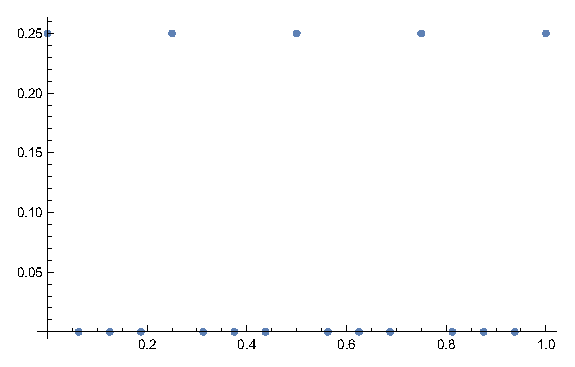
\includegraphics{img/Shor_gr1.eps}

\begin{doublespace}
\noindent\(\pmb{\text{(*Procesar medidas para tener la factorizaci{\' o}n*)}}\\
\pmb{\text{(*Fracciones continuas*)}}\\
\pmb{\text{L1}=\text{Table}[\{\text{Denominator}[\text{FromContinuedFraction}[\text{ContinuedFraction}[\text{Transpose}[L][[2,i]]]]],L[[i,3]]\},\{i,1,16\}];}\\
\pmb{\text{For}[i=1,i\leq \text{Dimensions}[\text{L1}][[1]],i\text{++},\text{For}[j=1,j\leq \text{Dimensions}[\text{L1}][[1]],j\text{++},\text{If}[\text{L1}[[i,1]]==\text{L1}[[j,1]]\&\&i\neq
j,\text{L1}[[i,2]]\text{+=}\text{L1}[[j,2]];}\\
\pmb{\text{L1}=\text{Drop}[\text{L1},\{j\}];]]]}\\
\pmb{\text{For}[i=1,i\leq \text{Dimensions}[\text{L1}][[1]],i\text{++},\text{If}[\text{OddQ}[\text{L1}[[i,1]]],\text{L1}=\text{Drop}[\text{L1},\{i\}];]]}\\
\pmb{\text{For}\left[i=1,i\leq \text{Dimensions}[\text{L1}][[1]],i\text{++},\text{If}\left[\text{Mod}\left[x^{\text{L1}[[i,1]]},M\right]\neq 1,\text{L1}=\text{Drop}[\text{L1},\{i\}];\right]\right]}\\
\pmb{\text{For}\left[i=1,i\leq \text{Dimensions}[\text{L1}][[1]],i\text{++},\text{If}\left[\text{GCD}\left[x^{\frac{\text{L1}[[1,1]]}{2}},M\right]==M-1,\text{L1}=\text{Drop}[\text{L1},\{i\}];\right]\right]}\\
\pmb{\text{For}\left[i=1,i\leq \text{Dimensions}[\text{L1}][[1]],i\text{++},\text{L1}[[i,2]]=\frac{\text{L1}[[i,2]]}{\text{Sum}[\text{L1}[[j,2]],\{j,1,\text{Dimensions}[\text{L1}][[1]]\}]};\right]}\\
\pmb{\text{L2}=\text{Table}\left[\left\{\text{GCD}\left[x^{\frac{\text{L1}[[i,1]]}{2}}+1,M\right],\text{L1}[[i,2]]\right\},\{i,1,\text{Dimensions}[\text{L1}][[1]]\}\right];}\\
\pmb{\text{L3}=\text{Table}\left[\left\{\text{GCD}\left[x^{\frac{\text{L1}[[i,1]]}{2}}-1,M\right],\text{L1}[[i,2]]\right\},\{i,1,\text{Dimensions}[\text{L1}][[1]]\}\right];}\)
\end{doublespace}

\begin{doublespace}
\noindent\(\pmb{\text{(*Graficar probabilidad de cada posible orden estimado*)}}\\
\pmb{\text{L1}}\\
\pmb{\text{ListPlot}[\text{L1}]}\)
\end{doublespace}

\begin{doublespace}
\noindent\(\{\{16,\text{5.200010849845537$\grave{ }$*${}^{\wedge}$-33}+0. i\},\{8,\text{6.162975822039155$\grave{ }$*${}^{\wedge}$-33}+0. i\},\{4,1.\,
+0. i\}\}\)
\end{doublespace}

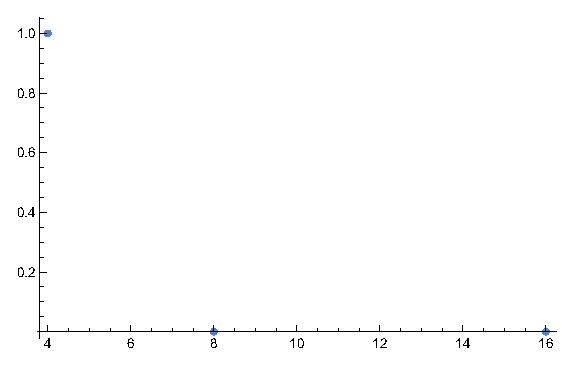
\includegraphics{img/Shor_gr2.eps}

\begin{doublespace}
\noindent\(\pmb{\text{(*Graficar la probabilidad de cada posible factorizaci{\' o}n hallada*)}}\\
\pmb{\text{L2}}\\
\pmb{\text{ListPlot}[\text{L2}]}\\
\pmb{\text{L3}}\\
\pmb{\text{ListPlot}[\text{L3}]}\)
\end{doublespace}

\begin{doublespace}
\noindent\(\{\{1,\text{5.200010849845537$\grave{ }$*${}^{\wedge}$-33}+0. i\},\{1,\text{6.162975822039155$\grave{ }$*${}^{\wedge}$-33}+0. i\},\{5,1.\,
+0. i\}\}\)
\end{doublespace}

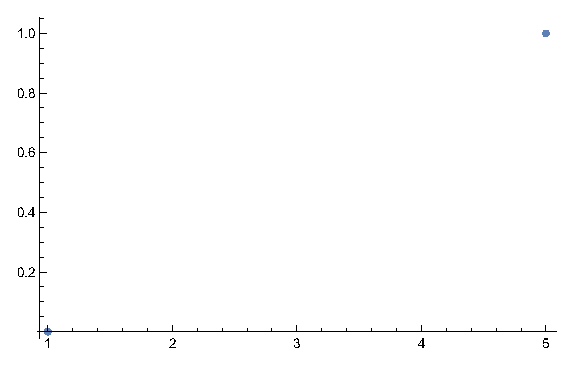
\includegraphics{img/Shor_gr3.eps}

\begin{doublespace}
\noindent\(\{\{15,\text{5.200010849845537$\grave{ }$*${}^{\wedge}$-33}+0. i\},\{15,\text{6.162975822039155$\grave{ }$*${}^{\wedge}$-33}+0. i\},\{3,1.\,
+0. i\}\}\)
\end{doublespace}

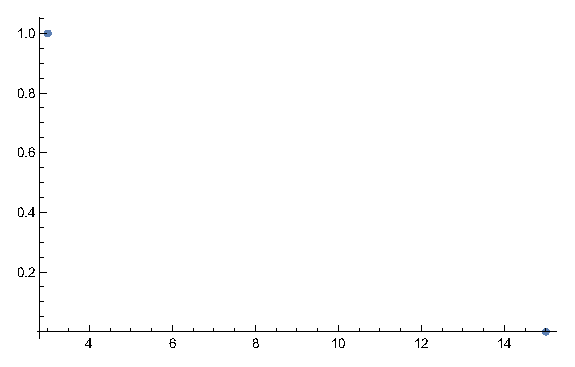
\includegraphics{img/Shor_gr4.eps}


\section{Simulación en Python}


\begin{verbatim}
import matplotlib.pyplot as plt
import matplotlib as mpl
import numpy as np
from scipy.stats import norm
from qutip import *
import tgates8
import time


#Transformada inversa de Fourier
def QFT4d(psi0, target1, target2, target3, target4):
    res = tgates8.SWAP(psi0, target2, target3)
    res = tgates8.SWAP(res.states[-1], target1, target4)
    res = tgates8.H(res.states[-1], target4)
    res = tgates8.CP(res.states[-1], target4, target3, -2*np.pi/2**2)
    res = tgates8.H(res.states[-1], target3)
    res = tgates8.CP(res.states[-1], target4, target2, -2*np.pi/2**3)
    res = tgates8.CP(res.states[-1], target3, target2, -2*np.pi/2**2)
    res = tgates8.H(res.states[-1], target2)
    res = tgates8.CP(res.states[-1], target4, target1, -2*np.pi/2**4)
    res = tgates8.CP(res.states[-1], target3, target1, -2*np.pi/2**3)
    res = tgates8.CP(res.states[-1], target2, target1, -2*np.pi/2**2)
    return tgates8.H(res.states[-1], target1)

#Compuerta de SWAP controlada
def CSWAP(psi0, control, target1, target2):
    res = tgates8.CCNOT(psi0, control, target1, target2)
    res = tgates8.CCNOT(psi0, control, target2, target1)
    return tgates8.CCNOT(psi0, control, target1, target2)

#Operador de multiplicación por 7 módulo 15 controlado
def CMUL7(psi0, control, target1, target2, target3, target4):
    res = tgates8.CNOT(psi0, control, target1)
    res = tgates8.CNOT(res.states[-1], control, target2)
    res = tgates8.CNOT(res.states[-1], control, target3)
    res = tgates8.CNOT(res.states[-1], control, target4)
    res = CSWAP(res.states[-1], control, target2, target3)
    res = CSWAP(res.states[-1], control, target1, target2)
    return CSWAP(res.states[-1], control, target1, target4)

#Dimensión del espacio de Hilbert
qN = 2**8


# El algoritmo
# Estado fiducial
psi0 = tensor(basis(2,0), basis(2,0), basis(2,0), basis(2,0),
              basis(2,0), basis(2,0), basis(2,0), basis(2,0))

# Preparación del estado inicial
res = tgates8.X(psi0, 7)

qsave(res, 'rp_0')

# Transformada de Hadamard en el primer registro
res = tgates8.H(res.states[-1], 0)
res = tgates8.H(res.states[-1], 1)
res = tgates8.H(res.states[-1], 2)
res = tgates8.H(res.states[-1], 3)

qsave(res, 'rp_1')

# Aplicando CMUL7(c=3)^1
res = CMUL7(res.states[-1], 3, 4, 5, 6, 7)

qsave(res, 'rp_2')

# Aplicando CMUL7(c=2)^2
res = CMUL7(res.states[-1], 2, 4, 5, 6, 7)
res = CMUL7(res.states[-1], 2, 4, 5, 6, 7)

qsave(res, 'rp_3')

# Aplicando CMUL7(c=1)^4
res = CMUL7(res.states[-1], 1, 4, 5, 6, 7)
res = CMUL7(res.states[-1], 1, 4, 5, 6, 7)
res = CMUL7(res.states[-1], 1, 4, 5, 6, 7)
res = CMUL7(res.states[-1], 1, 4, 5, 6, 7)

qsave(res, 'rp_4')

# Aplicando CMUL7(c=0)^8
res = CMUL7(res.states[-1], 0, 4, 5, 6, 7)
res = CMUL7(res.states[-1], 0, 4, 5, 6, 7)
res = CMUL7(res.states[-1], 0, 4, 5, 6, 7)
res = CMUL7(res.states[-1], 0, 4, 5, 6, 7)
res = CMUL7(res.states[-1], 0, 4, 5, 6, 7)
res = CMUL7(res.states[-1], 0, 4, 5, 6, 7)
res = CMUL7(res.states[-1], 0, 4, 5, 6, 7)
res = CMUL7(res.states[-1], 0, 4, 5, 6, 7)

qsave(res, 'rp_5')

# Aplicando la transformada cuántica inversa de Fourier sobre el primer registro
res = QFT4d(res.states[-1], 0, 1, 2, 3)

qsave(res, 'rp_6')

\end{verbatim}

\begin{figure}[H]
\centering 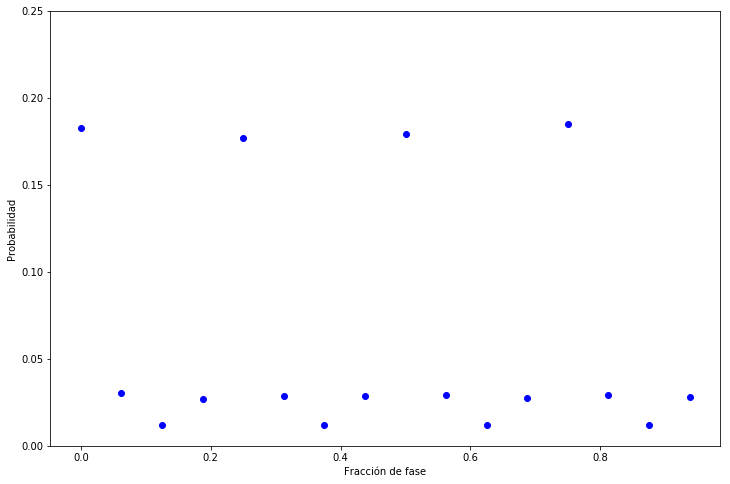
\includegraphics[width=0.9\linewidth]{img/shorlossless.png}
\caption{}
\end{figure}

[0.18265120316248348,
 0.030148605498127055,
 0.0117556126084082,
 0.027068348030583445,
 0.17700021614033762,
 0.028491802773181096,
 0.011881438650927171,
 0.028510782606300467,
 0.17917422966710292,
 0.029450553218688075,
 0.012081135256705483,
 0.027710388875941253,
 0.18489803932544116,
 0.02936951642045106,
 0.012035158723792341,
 0.027772969041529337]

